% !TEX root = ../thesis-example.tex
%
\section{Hyperledger-based Application}
\label{sec:impr:hl}

With the interfaces needed to easily expand the system being in place, we deemed it a good next step to add another Blockchain protocol. Specifically, we chose \emph{Hyperledger}. The application was successfully expanded with all necessary components built and tested, although the front-end still has problems trying to pack this new addition and sending it to the user's browser. This issue is elaborated in section \ref{sec:issues:integration}. This chapter will focus on firstly giving a broad overview of Hyperledger in section \ref{sec:impr:hl:basics} and then following up with detailing the implemented expansion in the later sections.

\subsection{Hyperledger as a Ledger Protocol}
\label{sec:impr:hl:basics}

To explain how the Systems of \emph{Hyperledger Fabric} work and what special features they offer, it makes sense to offer a comparison to the \emph{Ethereum} Blockchain - feature by feature. \emph{Hyperledger} wants to set itself apart by being a business-oriented information transfer protocol (hence, a shared ledger). Values, like tokens (e.g., \emph{Bitcoin, Ethereum}), are not a fundamental part of it.

\textbf{Authorization} \\[0.2em]
If configured, a Hyperledger Network will be split into groups, called organisations. Each organisation has a (potentially distinct) \emph{Certificate Authority (CA)}, through which membership in an organization is validated for every peer and account. Therefore, if one wants to interact with the network by for example invoking a smart contract, they must first be authenticated  by the CA. The CA even allows for group roles, so not every query to the network is accessible to everyone. These group roles were not further regarded in this task, however.

\textbf{Block Sealing} \\[0.2em]
Block sealing, the process of adding blocks to the Blockchain and therefore changing it's active state and log, is an essential part of Blockchain technology. In more known protocols like \emph{Bitcoin} or (at least at the time of writing) \emph{Ethereum}, the content of the next block is decided by the node that first managed to solve a cryptographic puzzle - the solving of this puzzle being called \emph{mining}. This, however, means that the time of sealing a block is somewhat random - and a bidding process is necessary to convince the block sealer of writing one's data. \newline
Hyperledger circumvents this competition-based method and instead introduces an \emph{orderer} node, which generally tries to apply block-additions in a first-in-first-out fashion (and accounts for concurrency issues). This means a more reliable way of querying the blockchain, since all actions are executed as fast as resources allow, and also because competing peers are treated equally instead of based on their bid. \newline
Additionally, from a security standpoint, a network can not as easily be 'poisoned' (by holding such a large amount of tokens or mining power that the holder can essentially decide which transactions to incorporate), since the finances and mining capacities of peers are disregarded completely.

\begin{figure}[h]
	\centering
	\captionsetup{justification=centering,margin=2cm}
	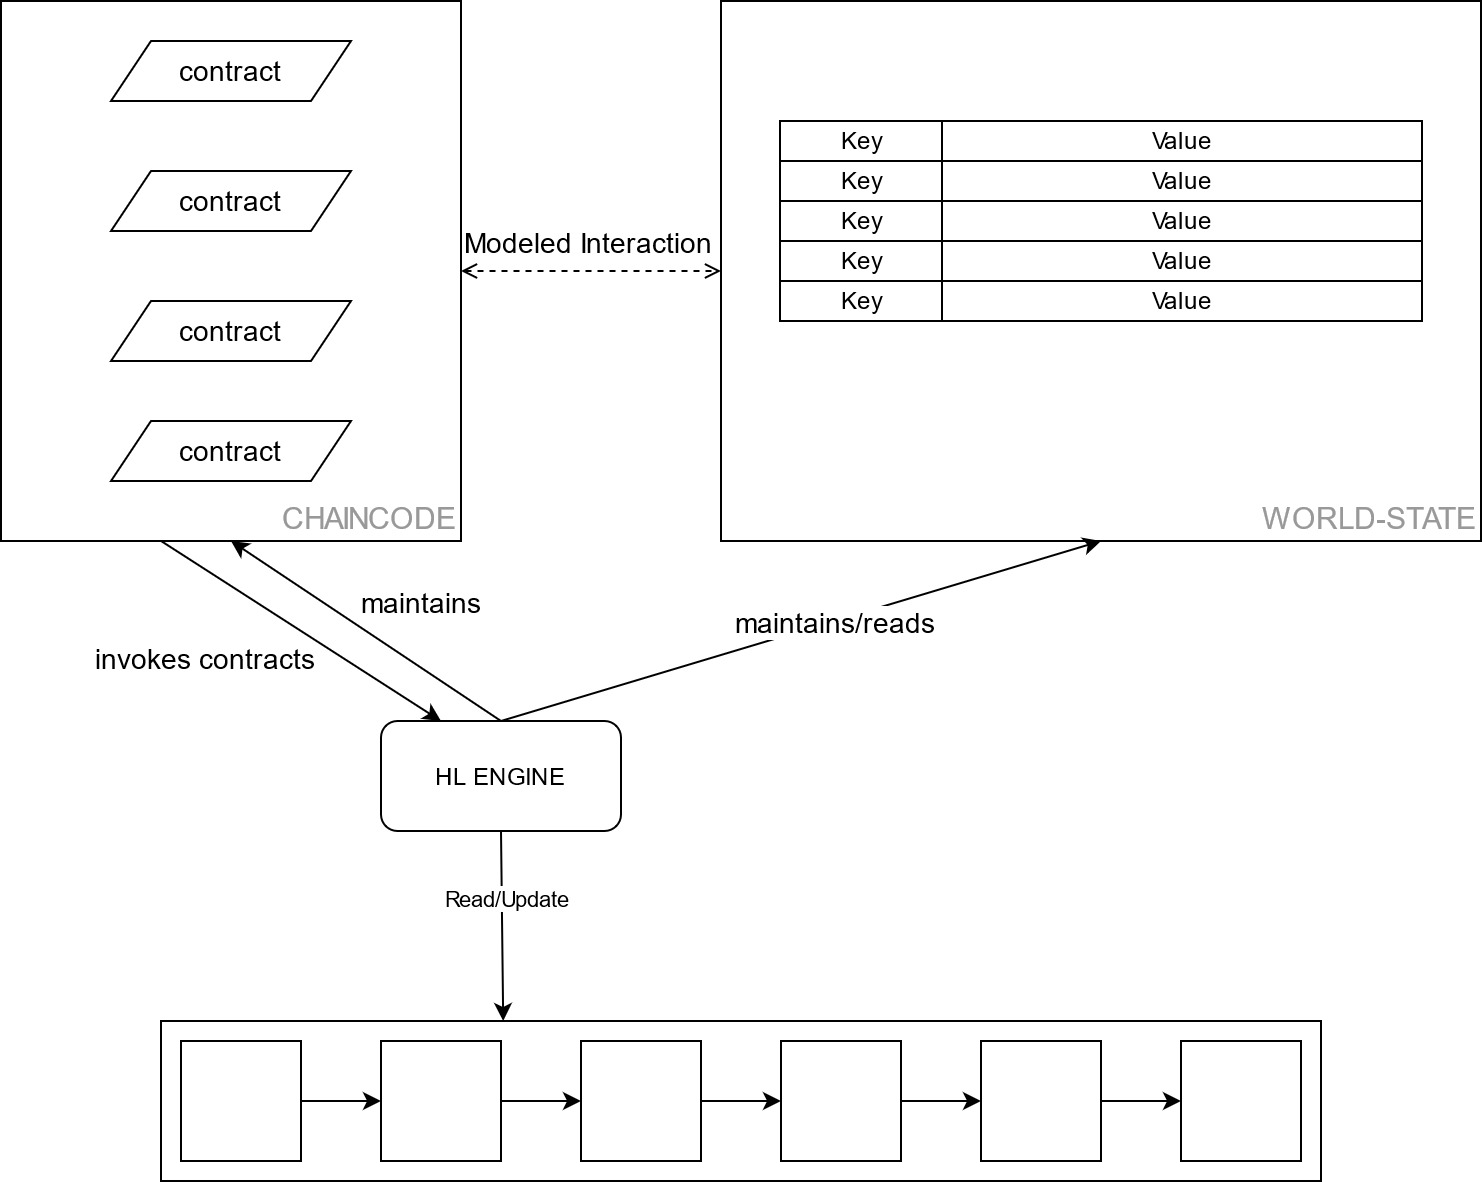
\includegraphics[height=0.7\textwidth]{gfx/hl-abstraction}
	\caption{Sketch of \emph{Hyperledger's} abstraction mechanism.}
	\label{fig:impr:hl:basics:abstraction}
\end{figure}

\textbf{Abstraction: \emph{World State \& Chaincode}} \\[0.2em]
As depicted in figure \ref{fig:impr:hl:basics:abstraction} by an 'engine' component (although this is a big simplification), Hyperledger has functions in place to display the underlying Blockchain's contents in a more abstract way, so that the user or developer doesn't need to bother with physical addresses, but may instead find them in a more human-readable format. \newline
The \emph{World State} Container is a synchronous representation of all data present in Hyperledger's underlying Blockchain, meaning that the data points present are always a representation their most recent update. Additionally, the World State is arranged like a dictionary, so that every structure inside is reachable by a key, defined by the user itself. This way, the programmer doesn't have to worry about physical addresses of the data. \newline
In the \emph{Chaincode} containers one can find the Smart Contract objects one would also find in other Blockchain application. However, these contracts are not stateful and therefore do not contain any data besides the location of the World State, where the data may be contained. In comparison, an \emph{Ethereum}-based contract may have private data and would therefore be stateful. Additionally, Chaincodes are also invocable via name, specifically by a combination of the parent contract name and the function that is to be executed.

\subsection{Required Components}
\label{sec:impr:hl:requirements}

\begin{figure}[h]
	\centering
	\captionsetup{justification=centering,margin=2cm}
	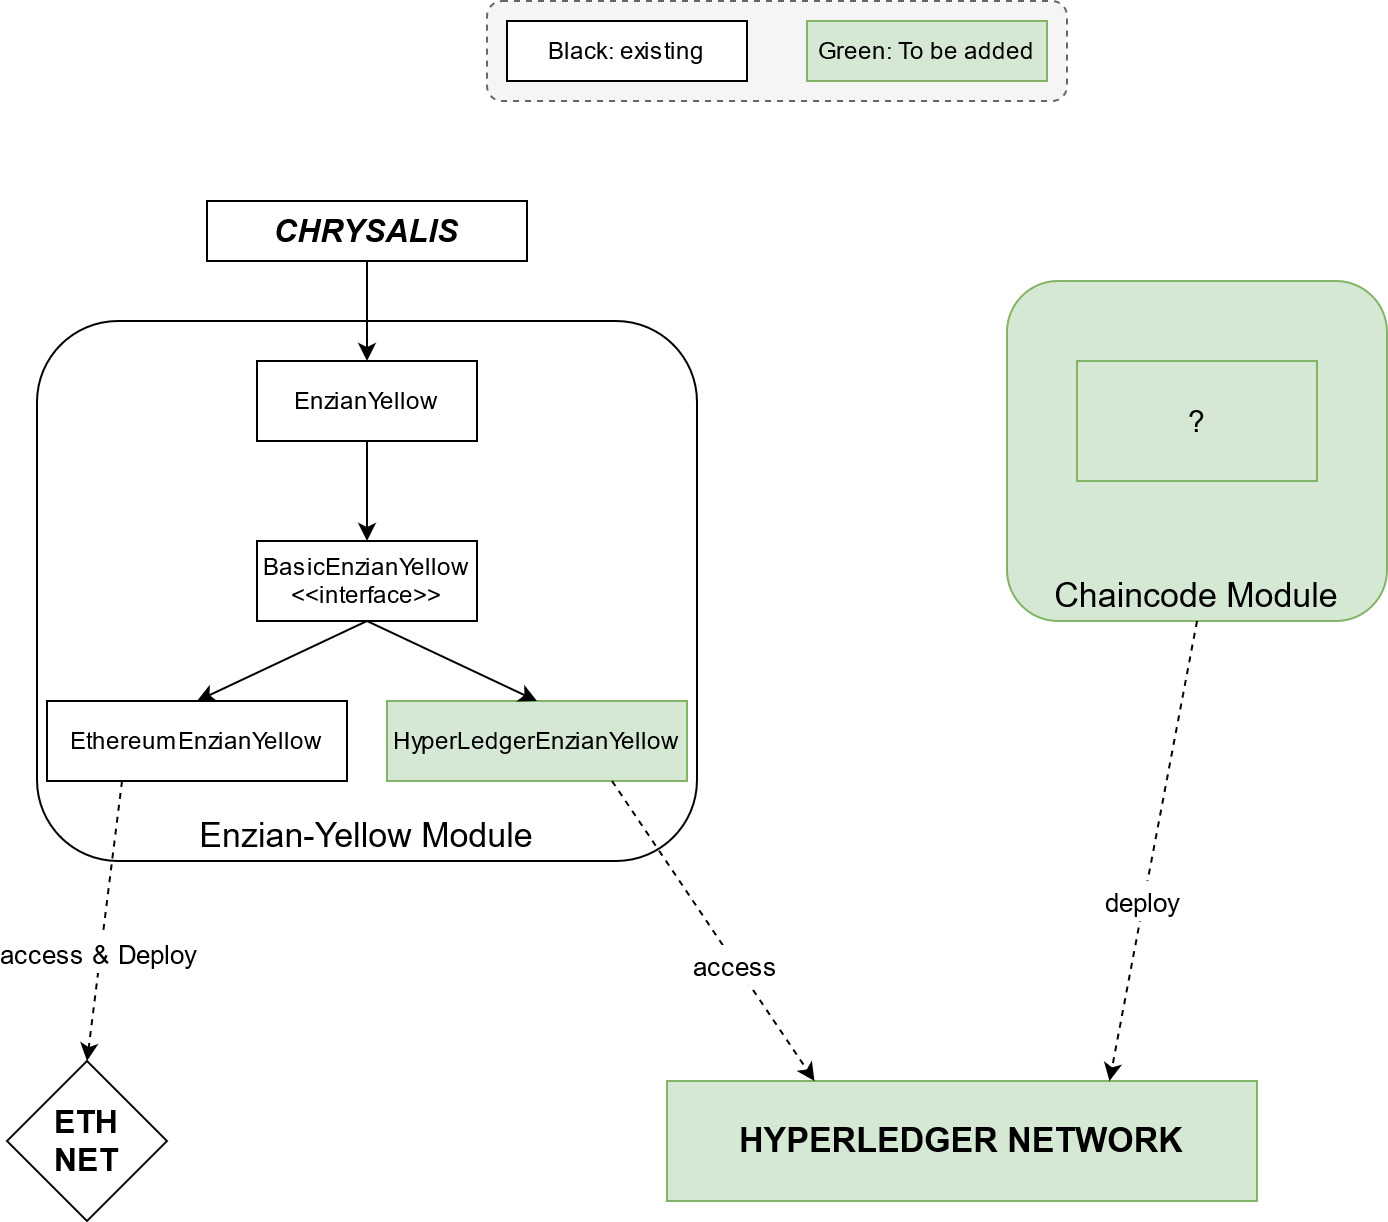
\includegraphics[width=\textwidth]{gfx/hl-structure}
	\caption{Planned and implemented module structure after adding the \emph{Hyperledger} protocol}
	\label{fig:impr:hl:structure}
\end{figure}

TODO explain what new components will appear and how they weave into EY

\subsection{Test-Network}
\label{sec:impr:hl:network}

TODO as in pres

\subsection{Representation of Processes}
\label{sec:impr:hl:datastructure}

TODO as in pres

\subsection{Process Deployment and Execution}
\label{sec:impr:hl:chaincode}

TODO as in pres

\subsection{Integration into Chrysalis}
\label{sec:impr:hl:integration}

TODO explain API a bit, otherwise as in pres

\subsection{Result}
\label{sec:impr:hl:result}

TODO mention issue